\section{Reachability Analysis on Hybrid Systems}

\subsection{Hybrid Automata}

Hybrid systems are a class of dynamical systems exhibiting both continuous flow and discrete jumps. They are usually systems composed of a discrete controller interacting with a physical environment. A popular class of formal models for hybrid systems are called \emph{hybrid automata}~\cite{Alur+/1995/hybrid_systems}, whose definition is given as follows.

\begin{defn}
 A \emph{hybrid automaton} is defined by a tuple $\mathcal{A} = \tupleof{\loc, \var, \flow, \trans, \inv, \init}$ such that
 \begin{itemize}[-]
  \item $\loc$ is a finite set which consists of all discrete locations (or modes) of the system,
  
  \item $\var$ is a finite set which contains all continuous variables of the system,
  
  \item $\flow$ is a function associating each location a continuous dynamics which is defined by an ODE,
  
  \item $\trans$ consists of finitely many discrete jumps among the locations. A jump from $\ell$ to $\ell'$ is defined by a tuple $\tupleof{\ell, G, R, \ell'}$ such that $G\subseteq \reals^{|\var|}$, $R: \reals^{|\var|}\rightarrow \reals^{|\var|}$ are called the \emph{guard} and \emph{reset} respectively. The jump is enabled, i.e., allowed to take place, only if the guard $G$ is satisfied by the variable values. After the jump is made, the variable values are reassigned according to the reset $R$.
  
  \item $\inv$ is a function that defines an \emph{invariant}, i.e., a valid variable value range, $\inv(\ell) \subseteq \reals^{|\var|}$ for each location $\ell \in \loc$,
  
  \item $\init$ is a set which contains all initial states of the system.
 \end{itemize}
\end{defn}

In the paper, we consider the jump guards defined by polynomial constraints, and jump resets defined by polynomial mappings.

\begin{example}
 We study the motion of a bouncing ball. We introduce the variable $x$ to denote the height of the ball and $v$ to denote its velocity. Initially, the ball is static and is at the position that is $5$m from the ground. Then it falls down due to gravity. When the ball hits the ground while falling, then it is bounced up, that is, the velocity is reversed immediately with some loss in the speed. Therefore, we need one location whose state space is at most a 2-dimensional Euclidean space. Since the height $x$ should always be non-negative, the invariant of the location is $\{(x',v')\,|\,x' \geq 0\}$. The continuous motion of the ball can be described by the ODE $\dot{x} = v$, $\dot{v} = -g$ wherein $g$ is the gravitational acceleration. The bouncing action can be modeled by a self-loop jump whose guard is $\{(x',v')\,|\,x' = 0 \wedge v' < 0\}$ and reset is $x' := x$, $v' = 0.8v$. Figure~\ref{fig:bouncing_ball} shows the hybrid automaton. In the rest of the paper, we omit the identity mapping(s) in a jump reset.
\end{example}

\begin{minipage}{0.48\textwidth}
 \centering
 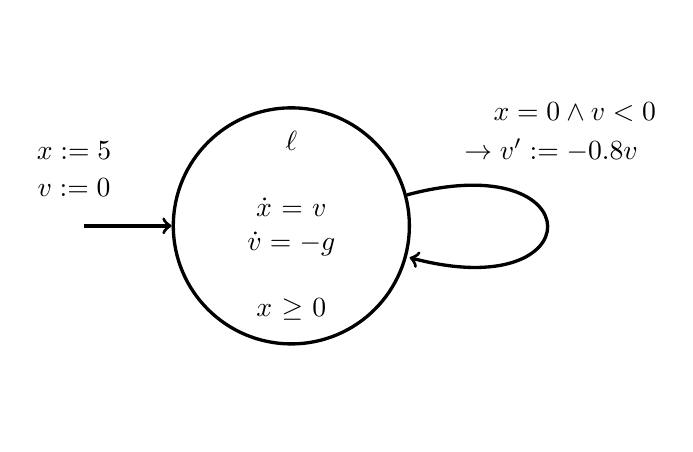
\begin{tikzpicture}[scale=1.2]
  \node[very thick, circle, text width=1.2cm, text centered, draw] (l) at (0,0) {$\ell$\\ \ \\ $\dot{x} = v$\\ $\dot{v} = -g$\\ \ \\ $x \geq 0$};
  \path[very thick, ->] (l) edge[loop right] (l);
  \node at (3,1.2) {$x = 0 \wedge v < 0$};
  \node at (2.75,0.8) {$\rightarrow v' := -0.8 v$};
  \node (dummy) at (-2.3,0) {};
  \path[very thick, ->] (dummy) edge (l);
  \node at (-2.3,0.8) {$x := 5$};
  \node at (-2.3,0.4) {$v := 0$};
  \node at (0,2) {};
  \node at (0,-2) {};
 \end{tikzpicture}
 \captionof{figure}{Hybrid automaton for a bouncing ball}\label{fig:bouncing_ball}
\end{minipage}
\hspace{1ex}
\begin{minipage}{0.48\textwidth}
 \centering
 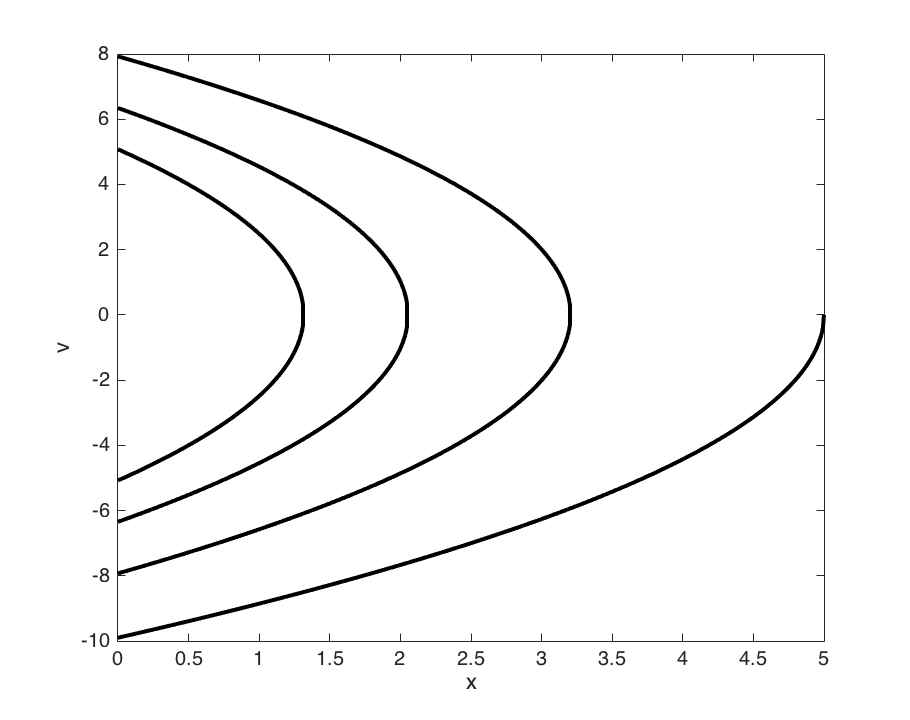
\includegraphics[height = 5cm]{images/bouncing_ball}
 \captionof{figure}{An execution of the hybrid automaton}\label{fig:execution}
\end{minipage}


A \emph{state} of a hybrid automaton $\mathcal{A}$ is denoted by a pair $(\ell, v)$ wherein $\ell$ is the current location and $v$ is a constant vector whose components denote the current values of the variables. A state $(\ell,v)$ can evolve to $(\ell', v')$ in the following two cases: (i) \emph{continuous evolution}, i.e., $\ell = \ell'$ and there is a solution $\varphi(t)$ of the ODE of $\ell$ such that $v = \varphi(t_1)$, $v' = \varphi(t_2)$, $t_1 \leq t_2$ and $\varphi(t) \in \inv(\ell)$ for all $t \in [0,t_2]$; (ii) \emph{discrete evolution}, i.e., there is a jump $\tupleof{\ell, G, R, \ell'}$ such that $v\in G$ and $v$ is updated to $v'$ according to $R$.

An \emph{execution} of a hybrid automaton is a sequence of states such that there is an evolution for each successive pair. As an example, Figure~\ref{fig:execution} illustrates an execution of the bouncing ball hybrid automaton over the time $[0,5]$. The trajectory is formed by line connecting each pair of successive states. Additionally, we call a state \emph{reachable} if it occurs in at least one execution of the system.




\subsection{Reachability Analysis}

The main task of reachability analysis is to check whether a given state is reachable or not. It plays a key role in the safety verification for systems, since if we can ensure that no unsafe state is reachable then the system is proved to be safe. However, checking the reachability of a state is not \emph{decidable} on hybrid automata (see~\cite{Alur+/1995/hybrid_systems}), we resort to computing an overapproximation for the system reachable state set.


In the paper, we use the tool \flowstar~\cite{Chen+/2013/flowstar} which computes Taylor model flowpipes for the hybrid automata with nonlinear dynamics. A \emph{Taylor model flowpipe} is an overapproximation of the reachable set in a small time period which is called a time step.


Taylor models are proposed by Berz and Makino as a replacement of intervals in rigorous computation (see~\cite{Berz/1999/Modern,Makino+Berz/2003/Taylor}). A Taylor Model (TM) is defined by a pair $(p,I)$ such that $p$ is a polynomial over a finite set of variables whose ranges are intervals, and $I$ is an interval. Given a continuous function $f(x)$ with $x\in D$ for some interval $D$. A TM (overapproximation) of it can be computed as $(p_f(x), I_f)$ such that $\forall x\in D.(f(x) \in p(x) + I)$. Usually, $p$ is a Taylor approximation of $f$ at the center of $D$ and $I$ is an interval enclosure of the remainder term. TMs are closed under operations such as addition, multiplication, and integration. Hence, a TM for a composed function can be computed based on the TMs of the components by TM arithmetic (see~\cite{Makino+Berz/2003/Taylor}).


In the rest of the section, we briefly introduce the approach of TM flowpipe construction. For hybrid automata, we need to compute the flowpipes under the two types of evolutions. The main framework is given by Algorithm~\ref{algo:hybrid_flowpipes}, and more details are also provided as follows.


\begin{algorithm}
 \caption{Flowpipe construction for hybrid automata}\label{algo:hybrid_flowpipes}
 \begin{algorithmic}[1]
  \REQUIRE{$\mathcal{A} = \tupleof{\loc, \var, \flow, \trans, \inv, \init}$, $T$, $k$.}
  \ENSURE{Overapproximation of the state set which are reachable in the time $[0,T]$ by at most $k$ jumps.}
  \STATE Add $\init$ to $\textit{Queue}$;
  \STATE $\mathcal{R} \leftarrow \emptyset$;
  \WHILE{$\text{Queue}$ is not empty}
   \STATE Dequeue the first state set in $\textit{Queue}$ and keep it as $S$;
   \STATE Compute the TM flowpipes from $S$ only under the continuous dynamics and add them to $\mathcal{R}$;
   \STATE Check the feasibility of all jumps in $\trans$;
   \STATE Compute a TM for the reachable set under each jump that is enabled;
   \STATE For each TM, if the corresponding time interval does not exceed $T$ and less than $k$ jumps executed previously, then add it to $\textit{Queue}$;
  \ENDWHILE
  \RETURN $\mathcal{R}$;
 \end{algorithmic}
\end{algorithm}


\noindent\textbf{Computing flowpipes under continuous dynamics.}
We use the technique named \emph{Taylor model integration} to compute overapproximations for the solutions of a nonlinear ODE with respect to a set of initial states. The main idea is explained as follows. Given an ODE $\dot{x} = f(\vx,t)$ and an initial condition $\vx(0) \in X_0$, we compute $N$ TM flowpipes $(p_1(\vx_0,t), I_1)$, $\dots$, $(p_N(\vx_0,t), I_N)$ with a time step size $\delta > 0$ to cover the time horizon $[0,N\delta]$, such that for $i=1,\dots,N$, the range of $(p_i(\vx_0,t), I_i)$ with $\vx_0\in X_0$ and $t\in [0,\delta]$ contains all ODE solutions in the time $[(i-1)\delta, i\delta]$, i.e., it is an overapproximation of the reachable set in the time $[(i-1)\delta, i\delta]$. The flowpipes are computed consecutively. More detains could be found in~\cite{Berz+Makino/1998/Verified, Chen/2015/phd}.

\todo{Add figures for flowpipes under continuous dynamics and jumps. }


\noindent\textbf{Feasibility checking for the jumps.}
When the TM flowpipes under the continuous dynamics are computed in a location $\ell$, we need to check the feasibility of all jumps starting from $\ell$. To do so, we check the validity of the formula $\exists i.\exists \vx_0.\exists t.(1\leq i\leq N \wedge \vx\in X_0 \wedge t\in [0,\delta] \wedge \vu\in I_i \wedge p_i(\vx_0,t) + vu) \in G$ for a guard $G$, i.e., at least one TM flowpipe has a non-empty intersection with $G$. Since the formula consists of nonlinear constraints which make it hard to solve exactly, we may resort to conservative methods such as Interval Constraint Propagation (ICP).




\noindent\textbf{Computing a TM reachable set overapproximation under a jump.}


